\input{wsc17style.tex}

\documentclass{wscpaperproc}

\usepackage{latexsym}
\usepackage{caption}
\usepackage{graphicx}
\usepackage{subcaption}
\usepackage[utf8]{inputenc}
\usepackage[table]{xcolor}

\usepackage[pdftex,
            colorlinks=true,
            urlcolor=blue,
            citecolor=black,
            anchorcolor=black,
            linkcolor=black] {hyperref}

\begin{document}

\WSCpagesetup{Ortega and Salgado}

\title{FARMERS, BANDITS AND SOLDIERS AN AGENT BASED SIMULATION ABOUT
       DELINQUENCY IN THE SOCIETY}

\author{Andrés Felipe Ortega Montoya\\ [12pt]
aortega7@eafit.edu.co\\
Ingeniería Matemática\\
Universidad EAFIT\\
\and
Alejandro Salgado Gómez\\[12pt]
asalgad2@eafit.edu.co\\
Ingeniería Matemática\\
Universidad EAFIT\\
}

\maketitle

\section*{ABSTRACT}
Delinquency is one of the main problems that societies face nowadays,
one the main reasons of this is the burden that it represents in the
economy and the effect that has in the life quality of the population.
This document describes the implementation of an agent base model that aims to
simulate a simplified version of a society and some of their interactions,
specifically those who have to do with the effects of delinquency.
In this work the society is conformed by three social groups, the
first one are farmers, that represent the productive class, the second
one are bandits, which represents the delinquency, and the last ones
are soldiers, that represents the public control. This work takes as base point
the ideas proposed in some articles of systems dynamics and adapt them to an
agent based simulation. As implementation tool we use the NetLogo software
\cite{netlogo}.

\section{Introduction}

Delinquency affects a lot of countries all around the world. Because of the
continuous problems that this actions generate in terms of social, economical and
political aspects, the nations continue to spend huge amount of resources
trying to keep this problematic as controlled as possible, but the results achieved
are poor, as seen in the indices of peace. Actually countries have become
less peaceful during the last decade, bringing enormous consequences to the
society. \cite{peace} \cite{violence}

With this motivation the authors developed an agent based model in which they
represent an artificial society that is conformed by three social groups,
Farmers, Bandits and Soldiers. The main objective of this model is to
analyze the effect of delinquency by testing different scenarios that
occur based on the configuration of the parameters of the simulation,
in order to see how this phenomenon affects the society and its
economy.

In the following sections we present some previous work that has been developed
in this topic, later a detailed description of the model its given, with the
help of the ODD (Overview, Design concepts and Details) methodology
\cite{modbook}, then an implementation section is introduced, there the details
of the creation process of the model will be explained. Lastly a section about
the experiments conducted with the model is shown and the conclusions of the
work are described at the end of the document.

\section{Previous work}

This work is based on two main articles, both addressed the problem from the
system dynamics perspective, however the authors find that the ideas proposed in
this articles can be applied in an agent base simulation, giving the possibility
to explore new characteristics of the problem and see others in a more
detail way, thanks to the granularity that this type of modeling offers.

The first article studies an artificial society where they seek for politics
that leads to a state of peace. In that work they represent the society with
the same groups as in the present work, and state that the members of the
society can change their role, based on psychological or economical conditions,
such as the level of empathy with their social group or the profits
that their occupations generate. The objective was to find politics
that leads to an stabilization of the system in a state of peace and
prosperity by changing different parameters of the model, such as the
sensibility to violence or the initial population of the different social
groups. \cite{article1}

The second article is about the confrontations between an insurgent force and
military forces of a government. In that work they describe the effects and
consequences about different strategies that can be used to try to solve the
problem, always with the goal of minimizing the threats civilians are exposed to.
This article states that one of the main factors that has to be taken
into account is the support that the population has to its government, because
this is the fact that defines if the civilian population will became part of the
insurgents rather than help the government, because it is in disagreement with
the actual state of the society. \cite{article2}

\section{Conceptual modeling}

\subsection{Generalities}

This model is the representation of a simplified society in which three types
of building define the infrastructure necessary for the interactions that occurs
between the three social groups. In this model the
economy is based on a single type of resource which represents all commodities,
this resources are produced by farmers in the first type of building named
farms, this buildings are assume as an infinite source of income. This
resources are also used as currency to pay taxes in the second type of
building, named city hall, this building represent the government
institutions and store the supplies that are used to sustain soldiers,
which are in charge of seeking for the well being of the farmers by
keeping bandit population at bay. The last building type, named houses,
are used by farmers and bandits to store the spare resources that they
earn either by gathering them in a farm, in the case of farmers, or
stealing, in the case of bandits.

\subsubsection{Purpose}

The purpose of the model is to analyze how delinquency affects the normal
development of a society, from the effect that has in the workforce and how
reactions, like incrementing the public force agents, emerge as response to
protect citizens from criminality.

\subsubsection{Entities and state variables}
\noindent \textbf{Entities}

\begin{itemize}
    \item Farms: Provides an endless source of the necessary resources for the
    population to subsist with.

    \item Houses: Serves as an storage for the spare resources an individual has
    after using a portion of those to meet its needs. If a given individual
    does not carry enough resources to refill its energy, they can use the
    ones they have previously stored in their house.

    \item City Hall: It stores the resources that farmers pay as taxes and also
    the ones soldiers seize from bandits. Soldiers can use the funds in the
    city hall to sustain themselves.

    \item Farmers: They gather resources from farms and pay a certain amount of
    those resources in the city hall as a way of paying soldiers for their
    protection.

    \item Bandits: Steal resources from farmers to sustain themselves while
    trying to avoid soldiers.

    \item Soldiers: Pursue bandits in order to reintegrate them into society as
    farmers and recover the funds they have stolen.
\end{itemize}

\newpage

\noindent \textbf{State variables}\\

\noindent The common attributes farmers, bandits and soldiers have are:

\begin{itemize}
    \item Energy: This serves as a way of telling of how much time an agent
    have before it needs to eat and thus return to its home or in the case or
    soldiers, city hall.

    \item Load: It represents the quantity of resources a given agent is
    carrying with itself at the moment.

    \item Destination: This is the current destination a given agent seeks to
    move towards to. In the case of farmers this can be their house, farm or
    city hall. In the case of bandits this can be a possible farmer to rob or
    their house. And finally it can be a nearby bandit or their city hall in
    the case of soldiers.
\end{itemize}

\noindent Houses and City Halls share a common attribute named inventory which
is the amount of resources it is storing at the moment.\hfill\break

\subsubsection{Process overview and scheduling}

Our process is divided in three parts, one for each social group. If the
agent is a farmer it will cycle through their assigned farm, city hall and
house. If the agent is a bandit will cycle trough, chasing after farmers trying
to assault them and going home. In the case of soldiers they loop over chasing
after bandits and going to their city hall. Finally on each tick all agents
will lose 1 unit of energy.

\subsection{Design concepts}

\subsubsection{Basic principles}

In this model it is supposed that the population is constant over time.  All
agents want to collect resources, each one in a different way depending on its
occupation. Also it is considered that there is a finite amount of weight and
energy that each individual can have. The supply of resources available on
farms and the amount of resources that can be stored in a building is taken
as infinite. Finally each person has their own house.

\subsubsection{Emergence}

There are many emergence behavior in the model like the agglomeration of
agents in some parts of the map as a consequence of various farmers being
assigned to the same workplace. This attracts bandits thus incrementing the
criminality nearby this places and therefore making soldiers to appear in this
zones. Also the appearance of sectors with a high density of bandits living in
it due to the remoteness that some places have from farms or city halls, making
the living as a farmer unsustainable.

\subsubsection{Adaptation}

In the model agents adapt to their current situation if the conditions does not
provides enough resources to supply for a living by means of changing their
occupation. It is important to notice that the social groups that an agent can
switch to depends on the occupation that they are currently performing.

\subsubsection{Objectives}

The objective of an agent varies depending on their current occupation. Farmers
try to collect as much resources as they can by working their respective farms.
Bandits try to steal as much resources from farmers as they can, trying not to
be captured by soldiers. Finally soldiers seek to decrease the amount of
bandits in the society.

\subsubsection{Learning}

Learning capabilities of agents are not taken into account in this model.

\subsubsection{Prediction}

Prediction procedures are not taken into account as part of the agent's
behavior in this model.

\subsubsection{Sensing}

In this model bandits can know which farmers are currently carrying any resources
with themselves, they also search for nearby soldiers in order to be ready to
run away. In the case of soldiers they can know the position of the closest
bandit, so that they can chase after it. Also all agents are aware of the
location of the necessary buildings to carry out their occupation.

\subsubsection{Interaction}

The model exhibit two types of interactions, one passive between members of the
social groups and the buildings, and the other one active between human agents
only. In the first case houses and city halls are used by active agents to
store their spare resources and farms are used by farmers to get the resources
they need for living. In the second case there are interactions between
bandits and the farmers they are going to steal from, and between soldiers and
the bandits they are seeking to convert.

\subsubsection{Stochasticity}

This model is present a stochastic behavior due to the random initialization of
buildings and the introduction of a fix probability to determine the change of
occupation in the case of farmers to simulate the government support they have.

\subsubsection{$\ \ $Collectives}

The model is define in terms of three major groups, farmers that represent
the productive class, bandits which represents the delinquency and soldiers
that represent control of the government in the society. The dynamic of the
system is define in terms of the interactions of these three groups.
% search for houses

\subsubsection{$\ \ $Observation}

The variables that are necessary to know the current state of the system are
the population of each social group. The violence indicator, which is defined
in terms of the number of crimes committed in a specific location of the map.
Finally the capital that each group is currently possessing, which describes the
economical force and hence the success that the group has achieved.

\subsection{Details}

\subsubsection{Initialization}

The model has 14 parameters, the first nine correspond to the population,
energy and max load of each social group. Also there are two parameters in
charge of setting the amount of city halls and farms that the simulation will
have. Another parameter is the energy from food, that defines the amount of
energy recovered by each unit of resource. There is another parameter name tax
rate that establishes the tax fee that farmers have to pay in the city halls.
Finally the government support parameter is used as the probability that a
farmer has to choose to become a bandit or a soldier when the choice arises.

At the begining of the simulation the position of all agents is chosen randomly
and all the parameters described above are used to determine the execution of
the simulation.

\subsubsection{Input}

There is no input data used in the model.

\subsubsection{Submodels}

\begin{itemize}
    \item \textbf{Move:} Is executed on each tick by all human agents, which
    will make them move to their current destination and lose 1 unit of energy.
    If they have no energy they will start consuming the resources they are
    carrying at the moment to supply their lack of energy.

    \item \textbf{Rest:} Is executed when an agent gets to
    their resting place (houses in the case of bandits and farmers, and city
    halls for soldiers) they will consume as much of the resources they
    have at their disposal to refill their energy. Any remaining resources will
    be stored in their resting place for later use. On the other hand, if they
    do not have enough resources to do so, they will execute the
    switch-occupation submodel.

    \item \textbf{Switch-occupation:} This one is executed in a different way
    depending on the agent occupation. In the case of farmers it will decide if
    the new occupation is to became a soldier or a bandit depending on the
    government support. For both bandits and soldiers it will cause them to
    switch occupation into farmers.

    \item \textbf{Work:} This submodel is unique for farmers. When it is
    executed they will extract resources from the farm they are currently in.
    The amount of resources extracted will be equal to the max load they are
    able to carry. Finally they will set their destination to the city hall to
    pay-taxes.

    \item \textbf{Pay-taxes:} This is also present only in farmers.
    They will pay as much resources of the tax rate parameter as they can. If
    they have less than the amount required they will give up all they
    have. Whatever the amount of resources they are able to give, will be stored
    in the city hall to pay for soldiers expenses. Lastly they will change
    their destination to home in order to rest.

    \item \textbf{Assault:} Only bandits are allowed to execute this submodel.
    They will set their destination to the nearest farmer with non-zero load to
    steal all of their belongings. In the case that there is a nearby soldier
    they will prioritize moving away from them to avoid being caught. They
    will continue to do so until either their energy hits zero or they get to the
    maximum amount of load they are able to carry, and later set their destination
    to their home in order to call the rest submodel.

    \item \textbf{Seize:} Finally, this submodel is responsible to make
    soldiers set their destination to the nearest bandit, if they get close
    enough, they will make them execute the switch-occupation submodel. All
    the resources bandits carry when they get caught are then seized by the
    soldier. They will chase after bandits until either their energy hits zero
    or they meet their maximum load, after which they will change their
    destination to the city hall to rest.

\end{itemize}

\section{Input data}

This model does not use any database for its implementation. The parameters
described in the last section are what defines how the simulation will execute.

\section{Implementation}

As mentioned before the model was implemented using the NetLogo software
\cite{netlogo}. The first element of the model is the simulation field
presented in figure \ref{imp:main_interface1} which shows the space distribution
of all agents. Farmers are blue, bandits are orange and soldiers are
green, just like their houses. Farms are shown in brown with the symbol of a cow
and city halls are presented with gray color and a colonial house symbol. All
agents show the amount of resources they have as a label on top of them. And the
red squares represent the danger zones, their color intensity is directly
proportional to how dangerous is the location.

\newpage

\begin{figure}[h!]
    \centering
    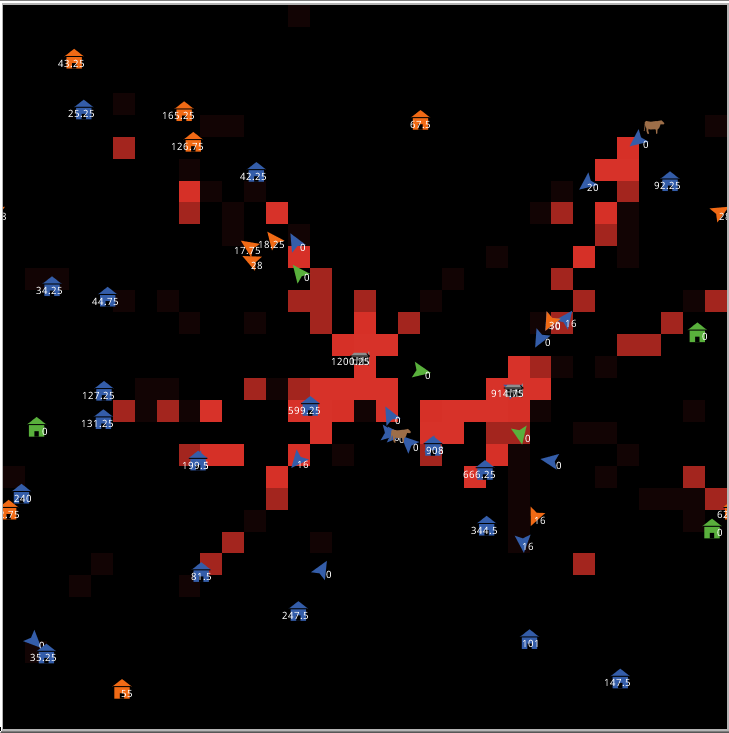
\includegraphics[scale=0.65]{Images/Interface1}
    \caption{Main interface}
    \label{imp:main_interface1}
\end{figure}

The second element of the interface are the economical and population indicators,
which are shown in figure \ref{imp:economy1} and figure
\ref{imp:population_plot1} respectively. They show the total inventory that
a specific group has stored in their respective buildings (houses for
farmers and bandits, and city halls for soldiers) and the number of
individuals per social group during all the execution.\\

\begin{figure}[h!]
    \centering
    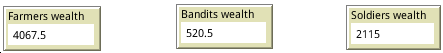
\includegraphics[scale=0.5]{Images/Economy1}
    \caption{Economy indicators}
    \label{imp:economy1}
\end{figure}

\begin{figure}[h!]
    \centering
    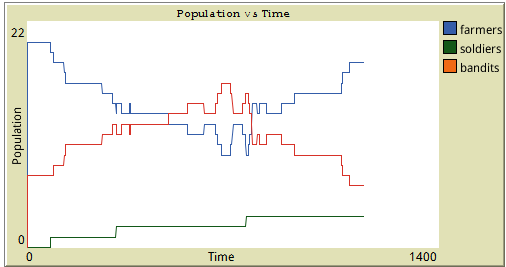
\includegraphics[scale=0.5]{Images/Population1}
    \caption{Population plot}
    \label{imp:population_plot1}
\end{figure}

In figure \ref{imp:parameters1} are shown all the parameters of the model as
sliders. The ``see danger zones" switch allows the user to see or hide the
danger measure of all locations.\\

\begin{figure}[h!]
    \centering
    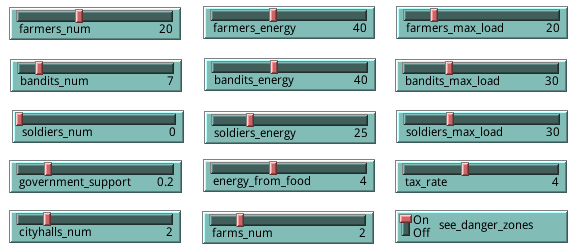
\includegraphics[scale=0.5]{Images/Sliders1}
    \caption{Model parameters}
    \label{imp:parameters1}
\end{figure}

Finally in figure \ref{imp:buttons} are shown the three buttons to control the
execution. The first one is used to initialize the model, the second one
executes one tick of the simulation and the last one execute the model
continuously.

\begin{figure}[h!]
    \centering
    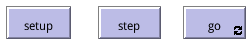
\includegraphics[scale=0.5]{Images/Buttons}
    \caption{Buttons to control execution}
    \label{imp:buttons}
\end{figure}

\section{Verification and validation}

After compare the results of the model with the ones shown in the reference
articles it was found that the model behaves as expected, even in cases with
extreme conditions, like the lack of some parameter or its full usage.

It is important to note that when a simulation is executed in multiple
times, the results may not be the same, this variations can be explained due
to the stochastic nature of the system and it is not because some failures in
the model.

Also its important to notice that this model is an extension of the original
implementation with a dynamic system perspective. In this work aspects like
the distribution of buildings or the energy of each human agent contributes
to make a more detail model, that can present results that contains those
aspects in a logic way, as it was expected, that can be use to understand what
its happening in the model.

\section{Experimentation}

In this section the results of some simulations are shown and a sensitivity
analysis es carried out. It is really important to highlight that, because
of the stochastic nature of the model, the results may not be reproduced
exactly. Most of the results shown are the average behavior of various
simulations.

\subsection{Results}

A variety of experiments were performed with the model. In figure
\ref{base_experiment} there is the base case of experimentation where the
population is composed mainly by farmers but there are some bandits in the
simulation, each group has the same amount of maximum energy but can carry
different amounts of resources, there is just a few city halls and farms, and
the government support and tax rate are low as well as the energy from food.
this simulation shows how the population of bandits starts to grows, until the
point that this group represents the majority of the society due to the great
profits that they can obtain from the unprotected farmers. But after a period
of time the system responds with the increment of soldiers, which generates the
decrease of bandits and takes the system to a state of peace.

\begin{figure}[h!]
    \begin{subfigure}{0.45\textwidth}
    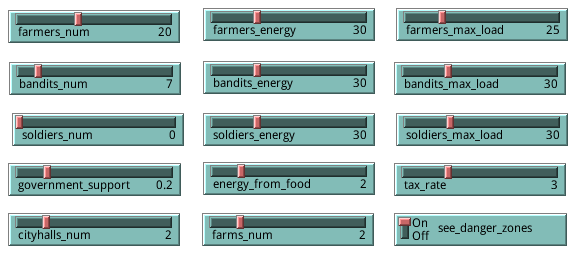
\includegraphics[width=\textwidth]{Images/Exp1_sliders.png}
    \caption{Experiment parameters}
    \end{subfigure}
    \hfill
    \begin{subfigure}{0.45\textwidth}
    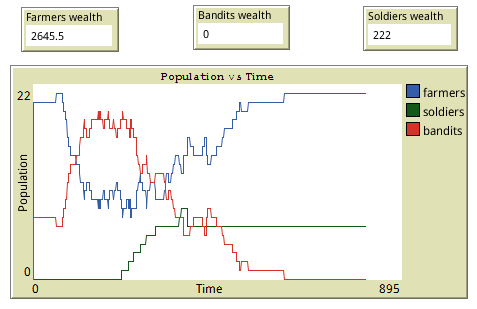
\includegraphics[width=\textwidth]{Images/Exp1_indicators.png}
    \caption{Experiment indicators}
    \end{subfigure}%
    \caption{Base case for experimentation}
    \label{base_experiment}
\end{figure}

In figure \ref{only_farmers} there is an experiment that aims to show the respond
of the model when the initial population is conformed exclusively of farmers. In
this simulation there are two cases, the first one, which is illustrated in the
figure, shows a period of stability at the beginning of the simulation, that is
later is disturbed because the distributions of buildings causes that
some houses are too far away from city halls or farms, which force
farmers to change their occupation, creating the dynamic represented. The other case
is when the distribution of buildings allows the farmers to generate enough
resources to live and therefore provokes a stabilization of the system in the
initial state.\\

\begin{figure}[h!]
    \begin{subfigure}{0.45\textwidth}
    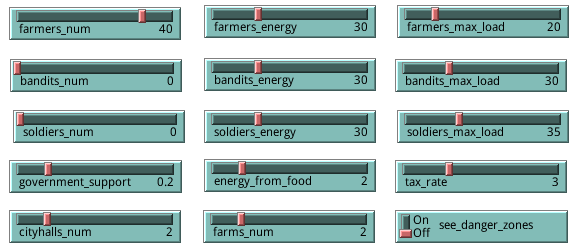
\includegraphics[width=\textwidth]{Images/Exp2_sliders.png}
    \caption{Experiment parameters}
    \end{subfigure}
    \hfill
    \begin{subfigure}{0.45\textwidth}
    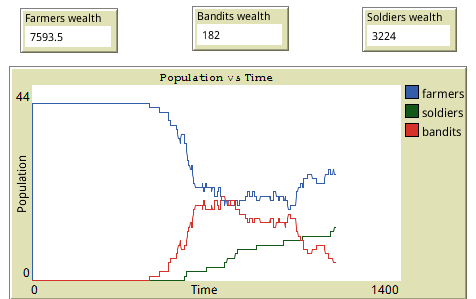
\includegraphics[width=\textwidth]{Images/Exp2_indicators.png}
    \caption{Experiment indicators}
    \end{subfigure}%
    \caption{Experiment with only farmers at the beginning of simulation}
    \label{only_farmers}
\end{figure}

Other cases can be found in figures \ref{bandits_only} and \ref{soldiers_only}
where the initial population is confirmed only by bandits. In this experiment
the behavior of the simulation is similar to the case presented above, there
is a period of stable execution followed by a great increment of farmers in
the system due to the fact that there is no resource production in the system.
At this point the same two cases of the past experiment reappear under the same
conditions and with the same consequences. Here the first case is shown in
figure \ref{bandits_only} and the second one is shown in figure
\ref{soldiers_only}.\\

\begin{figure}[h!]
    \begin{subfigure}{0.45\textwidth}
    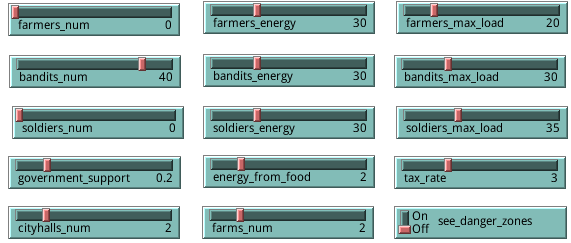
\includegraphics[width=\textwidth]{Images/Exp3_sliders.png}
    \caption{Experiment parameters}
    \end{subfigure}
    \hfill
    \begin{subfigure}{0.45\textwidth}
    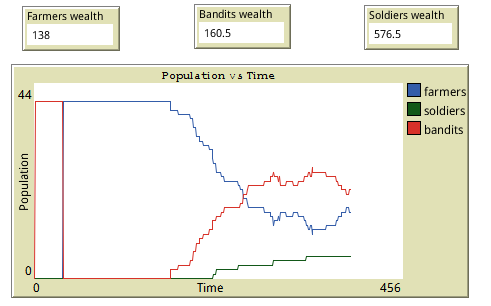
\includegraphics[width=\textwidth]{Images/Exp3_indicators.png}
    \caption{Experiment indicators}
    \end{subfigure}%
    \caption{Experiment with only bandits at the beginning of simulation}
    \label{bandits_only}
\end{figure}

\begin{figure}[h!]
    \begin{subfigure}{0.45\textwidth}
    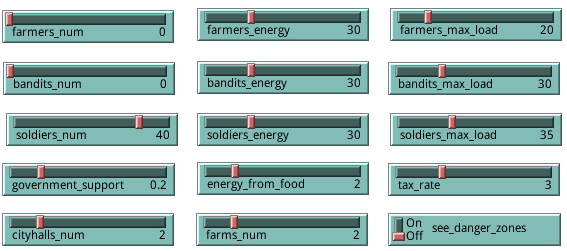
\includegraphics[width=\textwidth]{Images/Exp4_sliders.png}
    \caption{Experiment parameters}
    \end{subfigure}
    \hfill
    \begin{subfigure}{0.45\textwidth}
    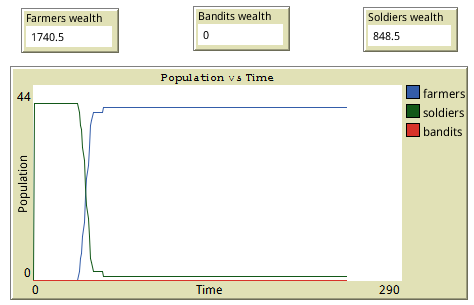
\includegraphics[width=\textwidth]{Images/Exp4_indicators.png}
    \caption{Experiment indicators}
    \end{subfigure}%
    \caption{Experiment with only soldiers at the beginning of simulation}
    \label{soldiers_only}
\end{figure}

\newpage

Finally in figure \ref{more_buildings} there is and experiment where the number
of farmers and city halls are incremented. This change generates that the farmers
can have such a profitable recollection of resources that (even with the presence
of some bandits in the system) the decrease of their revenue, either because of
tax payments or assaults, is not enough to make them change their occupation,
which causes a stabilization near the original setup of population distribution
in the system.

\begin{figure}[h!]
    \begin{subfigure}{0.45\textwidth}
    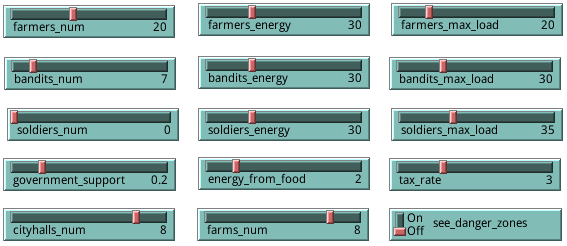
\includegraphics[width=\textwidth]{Images/Exp5_sliders.png}
    \caption{Experiment parameters}
    \end{subfigure}
    \hfill
    \begin{subfigure}{0.45\textwidth}
    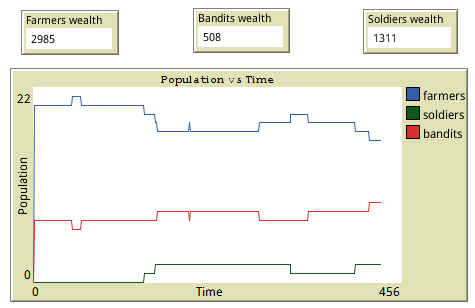
\includegraphics[width=\textwidth]{Images/Exp5_indicators.png}
    \caption{Experiment indicators}
    \end{subfigure}%
    \caption{Experiment with an increment in the number of farms and city halls}
    \label{more_buildings}
\end{figure}

\subsection{Sensitivity analysis}

The sensitivity analysis is performed for three parameters which are government
support, which represents the level of support that the civilian population has,
energy from food, that represents the amount the energy that each resource unit
provides. And finally the tax rate, representing the amount of resources that
the farmers have to pay in order to allow the soldiers to fulfill their mission.

The analysis is represented in tables \ref{table:government} to
\ref{table:taxes} and was carried based on the instructions found in
\cite{modbook}. The first row specifies the value of the parameter. The second
one shows the change that was performed, a positive value means an increment
and a negative value a decrement. The third parameter represents the number
of ticks necessary to decrease the population of bandits, and therefore the
delinquency, to a stable level close to zero, this value is taken as the
measure of each execution. Finally in the last row can be found the change of
the system respect to the change in the parameter.\\

Table \ref{table:government} shows the analysis of the first parameter. It was
found that the variation of this parameter has an important influence in the
simulations as it defines how inclined is the civilian population towards
delinquency. It is inversely proportional to the time that is necessary to
decrease delinquency near zero.

It is important to notice that the first value of that table is not a
contradiction because of its negative value. A negative value in the last
column indicates that the amount of ticks measured will change in an opposite
direction to the change in the parameter, which means that the first variation
of the table corresponds to a long execution time.\\

\begin{table}[h!]
    \centering
    \begin{tabular}{|c|c|c|c|}
        \hline
        Government support & Difference & Stabilization tick &  dC/dP\\
        \hline
        0.1 & -0.1 & 2525 & -1525\\
        \hline
        \rowcolor{lightgray}
        0.2 &      & 1762 & \\
        \hline
        0.3 & 0.1  & 1325 & -875\\
        \hline
        0.4 & 0.2  & 900 & -1725\\
        \hline
    \end{tabular}
    \caption{Sensitivity analysis for government support parameter}
    \label{table:government}
\end{table}

In table \ref{table:energy} can be found the analysis of the second
parameter. The experiments shown that the model is very sensible to this
parameter. It was found that the increment of its value will generate,
in an average case, a longer execution of the model, but it is hard to tell how
much influence is going to make in the simulation due to the stochastic
nature of the system.\\

\begin{table}[h!]
    \centering
    \begin{tabular}{|c|c|c|c|}
        \hline
        Energy from food & Difference & Stabilization tick &  dC/dP\\
        \hline
        2 & -2 & 800 & 1925\\
        \hline
        \rowcolor{lightgray}
        4 &      & 1762 & \\
        \hline
        6 & 2  & 6875 & 10225\\
        \hline
    \end{tabular}
    \caption{Sensitivity analysis for energy from food parameter}
    \label{table:energy}
\end{table}

Finally in table \ref{table:taxes} is the analysis of the third parameter. It
was found that the variation of the tax rate value is also inversely
proportional to the number of ticks that are necessary to reduce delinquency
towards zero. It is also important to notice that in a similar way than with
the first parameter, a reduction of this value will cause an increase in the
simulation time.\\

\begin{table}[h!]
    \centering
    \begin{tabular}{|c|c|c|c|}
        \hline
        Tax rate & Difference & Stabilization tick &  dC/dP\\
        \hline
        3 & -1 & 2800 & -4150\\
        \hline
        \rowcolor{lightgray}
        4 &    & 1762 & \\
        \hline
        5 & 1  & 1325 & -1750\\
        \hline
        6 & 2  & 1000 & -3050\\
        \hline
        7 & 3  & 975  & -3150\\
        \hline
        8 & 4  & 800  & -3850\\
        \hline
    \end{tabular}
    \caption{Sensitivity analysis for tax rate parameter}
    \label{table:taxes}
\end{table}

\section{Conclusions and recommendations}

\begin{itemize}
    \item The position of buildings is a key fact in the execution of the model.
\end{itemize}

\bibliographystyle{wsc}
\bibliography{entrega1}

\end{document}
